\section{Neutron Irradiation}
\label{sec:irradiation}

\subsection{Rhode Island Neutron Irradiation Facility}
\label{subsec:RINSC}
RINSC (Rhode Island Nuclear Science Center) is a 2 MW, light water cooled, pool type reactor in Narragansett, Rhode Island, USA.
At RINSC there are three (six?) different ways to irradiate materials: beamports (pipes that run from the work area to the reactor core), rabbit system (pneumatic system that ferries plastic sample bottles to the reactor core), and InCore tubes (small samples are placed into a tube and lowered into an empty basket next to the fuel elements). 
The beamports can accomodate samples of up to 7.75" x 3' [diameter by length], the rabbit system can accept sampes 1.125" x 6.25", and the InCore system can irradiate objects 1.25" x 9". 
Of the irradiation methods available, only the beamports are large enough to accomodate the silicon sensors for this project.
\begin{itemize}
    \item Fig 1 - image(s) of reactor core, beamport (see fig~\ref{fig:RINSC_Facility})
    what other details are useful here?
    \item Fig 2 - puck design/layout, real pucks (see fig~\ref{fig:Pucks_Arrayed})
    \item Fig 3 - puck layout, packing (see fig~\ref{fig:Puck_Packing})
    \item Fig 4 - other hardware, cylinder, temp monitoring setup
    \item Fig 5 - schemaitc of experimental setup? Is this needed?
    \item describe sample removal/storage after irradiation
    \item describe fluence measurement setup/procedure at Brown? 
\end{itemize}

  \begin{figure}[!hbt]
  \begin{center}
    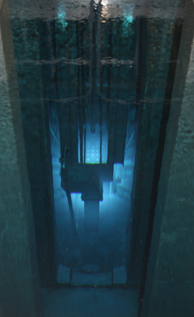
\includegraphics[width=0.25\textwidth]{figures/RINSC_Reactor_Core}
    \includegraphics[width=0.40\textwidth]{figures/Beamport_View}
    \caption{On the left is an image of the reactor core at RINSC, and on the right is a view down the beamport used for these irradiation studies.}
    \label{fig:RINSC_Facility}
  \end{center}
\end{figure}

\begin{figure}[!hbt]
  \begin{center}
    \includegraphics[width=0.70\textwidth]{figures/Hockey_Pucks_Arrayed}
    \caption{Sample containers ('hockey pucks') for sensors to be irradiated in the beamport at RINSC. The materials are wood (oak), acrylic, and PEEK.}
    \label{fig:Pucks_Arrayed}
  \end{center}
\end{figure}

  \begin{figure}[!hbt]
  \begin{center}
    \includegraphics[width=0.25\textwidth]{figures/Hockey_Puck_Base_Instrumented}
    \includegraphics[width=0.25\textwidth]{figures/Hockey_Puck_Sensor_Fit}
    \includegraphics[width=0.25\textwidth]{figures/Hockey_Puck_Kapton_Layer}
    \includegraphics[width=0.25\textwidth]{figures/Hockey_Puck_Lid_Instrumented}
    \caption{Four views of sensor container packing: the base instrumented with fluence monitoring diodes, the fit of a sensor in the hockey puck, the protection of the sensor with layers of kapton foil, and the lid of the hockey puck instrumented with monitoring devices.}
    \label{fig:Puck_Packing}
  \end{center}
\end{figure}

\subsection{List of Neutron-Irradiated Sensors}
\begin{itemize}
  \item full table of sensors irradiated in first campaign. Do we want to include sensors irradiated prior to the main campaign? On the order of 10 or so sensors maximum.
\label{subsec:sensors_irradiation}
